80. \begin{figure}[ht!]
\center{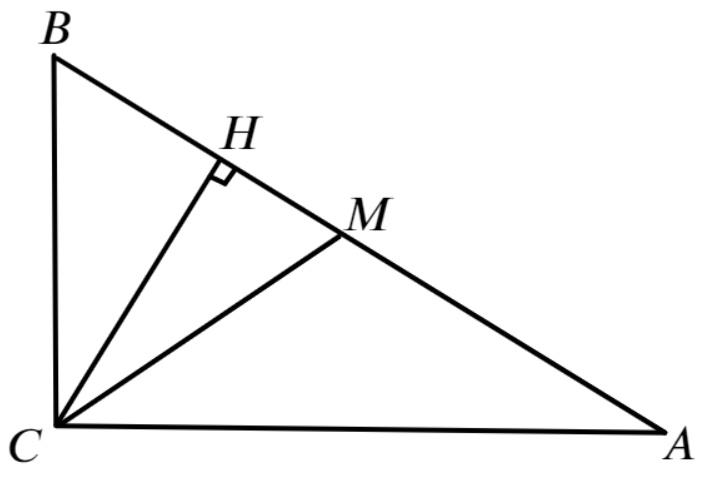
\includegraphics[scale=0.35]{g9-80.png}}
\end{figure}\\
Найдём $\angle B=90^\circ-24^\circ=66^\circ.$ Тогда $\angle BCH=90^\circ-66^\circ=24^\circ.$ Медиана, проведённая из прямого угла, равна половине гипотенузы, поэтому $CM=MA,$ а значит $\angle MCA=\angle A=24^\circ.$ Таким образом, $\angle HCM=90^\circ-24^\circ-24^\circ=42^\circ.$\\
